% File: T.tex
% Created: 2014-11-07
% Author: Tesser Paolo
% Email: p.tesser921@gmail.com
%
%
% Modification History
% Version	Modifier Date	Author			Change
% ====================================================================
% 0.0.1		2014-11-07		Tesser-Paolo	inserita sezione
% ====================================================================
% 0.0.2		2015-03-18		Tesser Paolo	inserito vocabolo: Tecniche di analisi
% ====================================================================
%

\section{T} % (fold)
\label{sec:t}
	\begin{itemize}
		\item \textbf{Tecniche di analisi}: [IS] ci sono diversi approcci per analizzare i bisogni e le fonti di un progetto. Attraverso lo studio del dominio, andando quindi ad osservare i comportamenti dell'utente finale e dell'ambiente d'uso immergendosi nei panni degli utilizzatori. Interagendo con il cliente in maniera il meno invasiva possibile e facendolo in modo strutturato e rendicontabile. Un'altra tecnica è quella di avere dei brain-storming, ma per farlo bisogna che:
			\begin{itemize}
				\item ci sia un gruppo di persone che sono consapevoli di ciò che stanno facendo;
				\item serve un'altra persona che fa da controllore, fissa l'agenda, il tempo e la scaletta;
				\item serve una persona che tenga le minute, cioè i punti salienti.
			\end{itemize}
		\noindent
		Infine può essere fatta anche della prototipazione, che può essere interna (per capire meglio le cose) o esterna (per chiedere al cliente se ciò che sta domandando);

		\item \textbf{Test}: [VV][analisi dinamica]
			\begin{figure}[htbp]
				\centering
				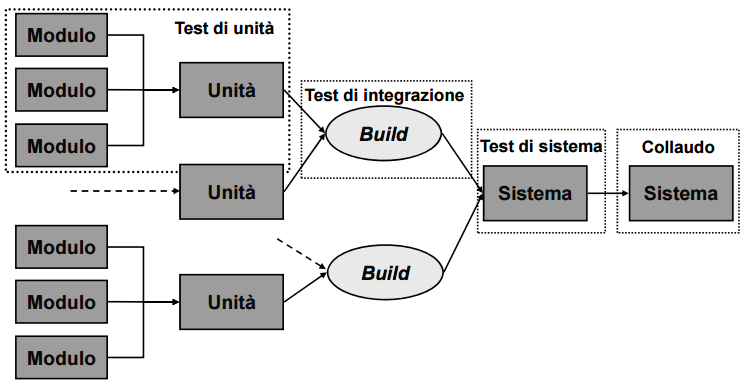
\includegraphics[scale=0.5]{img/composizione_test.png}
				\caption{Composizione Test}
				\label{fig:comp_test}
			\end{figure}

			\begin{itemize}
				\item \textbf{test di unità}: attività di analisi dinamica che se può svolgere con il massimo grado di parallelismo in quanto coinvolge la più piccola parte non ulteriormente scomponibile di un programma. La responsabilità è dello stesso programmatore per le unità più semplici, altrimenti di un verificatore autonomo. Nel primo caso infatti potrebbe esserci conflitto di interesse, meglio quindi peer-programming;
				\item \textbf{test di integrazione}: servono per verificare la costruzione incrementale del sistema. Può essere in parallelo per i componenti che non collaborano tra di loro. In condizioni ottimali, l'integrazione dovrebbe essere prova di problemi;
				\item \textbf{test di sistema e collaudo}: i primi sono svolti internamente dal fornitore per accertare la copertura dei requisiti SW, mentre i secondi sono supervisionati dal committente per dimostrare la conformità del prodotto sulla base di casi di prova specificati nel o implicati dal contratto;
				\item \textbf{test di regressione}: rappresentano l'insieme di test necessari ad accertare che la modifica di una parte P di S non causi errori in P o nelle altre parti di S che dipendono da P. Il rischio che degli errori si verifichino cresce tanto più cresce l'accoppiamento fra le diverse parti e al diminuire dell'accoppiamento.

			\end{itemize}







		\item \textbf{Tracciamento dei requisiti}: [DOC] ha il compito di fissare le relazioni tra i prodotti del processo di sviluppo. Vengono usate delle matrici di tracciabilità. Il tracciamento viene fatto in avanti (forward) che indica la completezza e all'indietro (backward) che indica la necessità. I tracciamenti necessari sono i seguenti:
			\begin{itemize}
				\item requisiti utente (capitolato) <-> requisiti software (AdR)
				\item requisiti software <-> descrizione dei componenti (ST)
				\item test di unità <-> moduli di disegno di dettaglio (DdP)
				\item test di integrazione <-> componenti architetturali
				\item test di sistema <-> requisiti software
				\item test di accettazione <-> requisiti utente
			\end{itemize}

	\end{itemize}
% section t (end)